%Este trabalho está licenciado sob a Licença Atribuição-CompartilhaIgual 4.0 Internacional Creative Commons. Para visualizar uma cópia desta licença, visite http://creativecommons.org/licenses/by-sa/4.0/deed.pt_BR ou mande uma carta para Creative Commons, PO Box 1866, Mountain View, CA 94042, USA.

\chapter{Superfícies Quádricas}\label{cap_superquad}
\thispagestyle{fancy}

Neste capítulo, fazemos um estudo introdutório sobre superífices quádricas.

\section{Introdução a superfícies quádricas}\label{cap_superquad_sec_intro}

Superfícies no espaço que podem ser descritas por equações da forma
\begin{equation}
  ax^2 + by^2 + cz^2 + 2dxy + 2exz + 2fyz + mx + ny + pz + q = 0
\end{equation}
são chamadas de \emph{superfícies quádricas}, sendo $a$, $b$, $c$, $d$, $e$, $f$, $m$, $n$, $p$ e $q$ coeficientes dados.

\subsection{Elipsoides}

Um \emph{elipsoide} centrado na origem é uma superfície quádrica de equação
\begin{equation}
  \frac{x^2}{a^2} + \frac{y^2}{b^2} + \frac{z^2}{c^2} = 1.
\end{equation}

\begin{ex}
  A Figura \ref{fig:sq_ex_elipsoide} é um esboço do gráfico da elipsoide de equação
  \begin{equation}\label{eq:sq_ex_elipsoide}
    \frac{x^2}{9} + \frac{y^2}{4} + z^2=1.
  \end{equation}
  
  \begin{figure}[H]
    \centering
    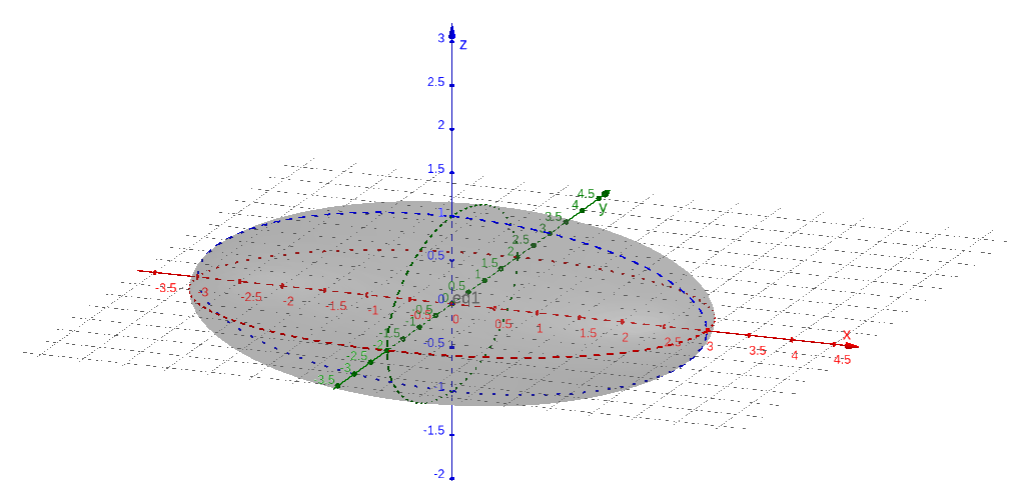
\includegraphics[width=\textwidth]{./cap_superquad/dados/fig_sq_ex_elipsoide/fig}
    \caption{Esboço do elipsoide de equação \eqref{eq:sq_ex_elipsoide}.}
    \label{fig:sq_ex_elipsoide}
  \end{figure}

  Observamos que a interseção deste elipsoide com o plano $X-Y$ (z=0) é a elipse de equação
  \begin{equation}
    \frac{x^2}{9}+\frac{y^2}{4}=1.
  \end{equation}
  Ou seja, é a elipse de vértice sobre o eixo maior $A_1=(-3,0)$ e $A_2=(3,0)$ e vértices sobre o eixo menor $B_1=(-2,0)$ e $B_2=(2,0)$.

  De forma análoga, temos que a interseção do elipsoide \eqref{eq:sq_ex_elipsoide} com o plano $X-Z$ ($y=0$) é a elipse de equação reduzida
  \begin{equation}
    \frac{x^2}{9} + z^2 = 1.
  \end{equation}
  Também, temos associada a elipse de equação reduzida
  \begin{equation}
    \frac{y^2}{4}+z^2=1
  \end{equation}
  que é obtida da interseção do elipsoide \eqref{eq:sq_ex_elipsoide} com o plano $Y-Z$ ($x=0$).  
\end{ex}

\subsection{Hiperboloides}

\subsubsection{Hiperboloides de uma folha}

Um hiperboloide de uma folha centrado na origem é uma superfície quádrica de equação
\begin{equation}
  \frac{x^2}{a^2}+\frac{y^2}{b^2}-\frac{z^2}{c^2}=1
\end{equation}
ou
\begin{equation}
  \frac{x^2}{a^2}-\frac{y^2}{b^2}+\frac{z^2}{c^2}=1
\end{equation}
ou
\begin{equation}
  -\frac{x^2}{a^2}+\frac{y^2}{b^2}+\frac{z^2}{c^2}=1
\end{equation}

\begin{ex}
  Vamos considerar o hiperboloide de equação
  \begin{equation}\label{eq:sq_ex_hiperboloide_z}
    \frac{x^2}{9}+\frac{y^2}{4}-z^2=1.
  \end{equation}
  Sua interseção com o plano $X-Y$ ($z=0$) é a elipse
  \begin{equation}
    \frac{x^2}{9}+\frac{y^2}{4}=1.
  \end{equation}
  Sua interseção com o plano $X-Z$ (y=0) é a hipérbole de equação reduzida
  \begin{equation}
    \frac{x^2}{9}-z^2=1.
  \end{equation}
  E, a interseção do hiperboloide com o plano $Y-Z$ ($x=0$) é a hipérbole de equação
  \begin{equation}
    \frac{y^2}{4}-z^2=1.
  \end{equation}
  
  A Figura \ref{fig:sq_ex_hiperboloide_z} é o esboço do gráfico do hiperboloide de equação \eqref{eq:sq_ex_hiperboloide_z}.

    \begin{figure}[H]
    \centering
    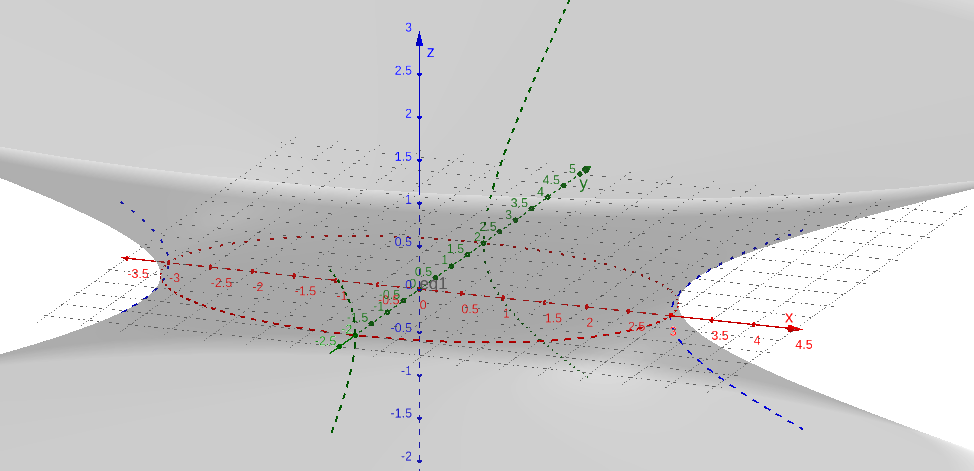
\includegraphics[width=\textwidth]{./cap_superquad/dados/fig_sq_ex_hiperboloide_z/fig}
    \caption{Esboço do hiperboloide de equação \eqref{eq:sq_ex_hiperboloide_z}.}
    \label{fig:sq_ex_hiperboloide_z}
  \end{figure}
\end{ex}

\begin{ex}
  A Figura \ref{fig:sq_ex_hiperboloide_x} é o esboço do gráfico do hiperboloide de equação
  \begin{equation}\label{eq:sq_ex_hiperboloide_x}
    -\frac{x^2}{9}+\frac{y^2}{4}+z^2=1.
  \end{equation}

  \begin{figure}[H]
    \centering
    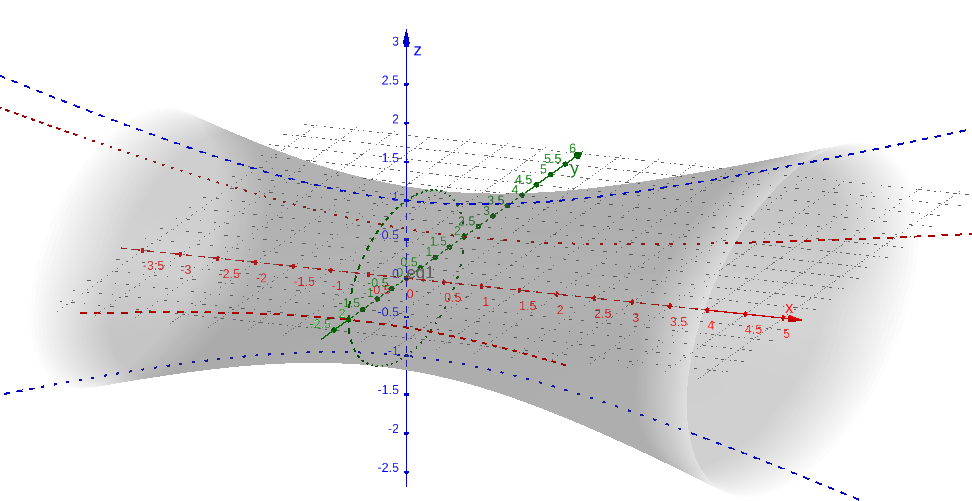
\includegraphics[width=\textwidth]{./cap_superquad/dados/fig_sq_ex_hiperboloide_x/fig}
    \caption{Esboço do hiperboloide de equação \eqref{eq:sq_ex_hiperboloide_x}.}
    \label{fig:sq_ex_hiperboloide_x}
  \end{figure}
  
  
  Sua interseção com o plano $X-Y$ ($z=0$) é a hipérbole
  \begin{equation}
    -\frac{x^2}{9}+\frac{y^2}{4}=1.
  \end{equation}
  Sua interseção com o plano $X-Z$ (y=0) é a hipérbole de equação reduzida
  \begin{equation}
    -\frac{x^2}{9}+z^2=1.
  \end{equation}
  E, a interseção do hiperboloide com o plano $Y-Z$ ($x=0$) é a elipse de equação
  \begin{equation}
    \frac{y^2}{4}+z^2=1.
  \end{equation}
\end{ex}

\subsubsection{Hiperboloides de duas folhas}

Hiperboloides de duas folhas têm equações
\begin{equation}
  \frac{x^2}{a^2}-\frac{y^2}{b^2}-\frac{z^2}{c^2}=1
\end{equation}
ou
\begin{equation}
  -\frac{x^2}{a^2}+\frac{y^2}{b^2}-\frac{z^2}{c^2}=1
\end{equation}
ou
\begin{equation}
  -\frac{x^2}{a^2}-\frac{y^2}{b^2}+\frac{z^2}{c^2}=1
\end{equation}

\begin{ex}
  Vamos considerar o hiperboloide de equação
  \begin{equation}\label{eq:sq_ex_hiperboloide_2f_x}
    \frac{x^2}{9}-\frac{y^2}{4}-z^2=1.
  \end{equation}
  Sua interseção com o plano $X-Y$ ($z=0$) é a hipérbole
  \begin{equation}
    \frac{x^2}{9}-\frac{y^2}{4}=1.
  \end{equation}
  Sua interseção com o plano $X-Z$ (y=0) é a hipérbole de equação reduzida
  \begin{equation}
    \frac{x^2}{9}-z^2=1.
  \end{equation}
  E, a interseção do hiperboloide com o plano $Y-Z$ ($x=0$) é vazia, pois não existem $y$ e $z$ que satisfazem a equação
  \begin{equation}
    -\frac{y^2}{4}-z^2=1,
  \end{equation}
  
    A Figura \ref{fig:sq_ex_hiperboloide_2f_x} é o esboço do gráfico do hiperboloide de equação \eqref{eq:sq_ex_hiperboloide_2f_x}.

    \begin{figure}[H]
    \centering
    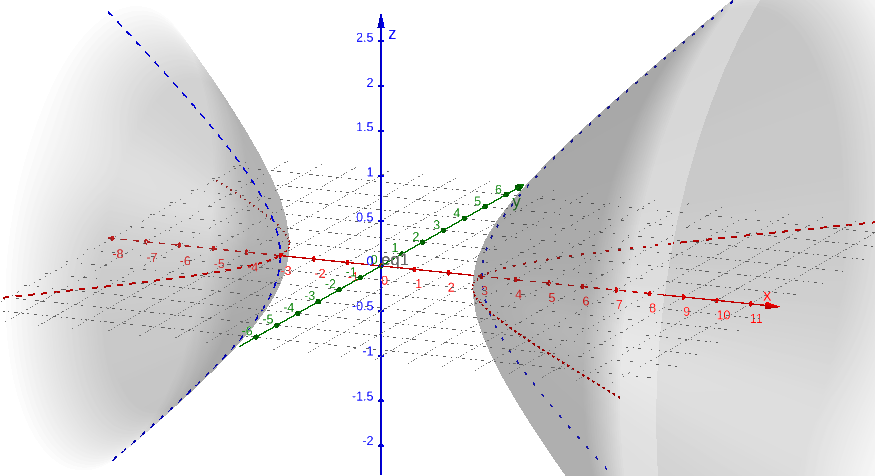
\includegraphics[width=\textwidth]{./cap_superquad/dados/fig_sq_ex_hiperboloide_2f_x/fig}
    \caption{Esboço do hiperboloide de equação \eqref{eq:sq_ex_hiperboloide_2f_x}.}
    \label{fig:sq_ex_hiperboloide_2f_x}
  \end{figure}
\end{ex}

\subsection{Paraboloide elíptico}

Um paraboloide elíptico tem equação
\begin{equation}
  \pm z = \frac{x^2}{a^2} + \frac{y^2}{b^2}
\end{equation}
ou
\begin{equation}
  \pm y = \frac{x^2}{a^2} + \frac{z^2}{c^2}
\end{equation}
ou
\begin{equation}
  \pm x = \frac{y^2}{b^2} + \frac{z^2}{c^2}
\end{equation}

\begin{ex}
  Vamos considerar o paraboloide elíptico de equação
  \begin{equation}\label{eq:sq_ex_parelip_z}
    z = \frac{x^2}{9}+\frac{y^2}{4}
  \end{equation}
  Não há valor $z<0$ que satisfaça a equação \eqref{eq:sq_ex_parelip_z}. Sua interseção com o plano $X-Y$ ($z=0$) é o ponto $(0, 0, 0)$. Agora, sua interseção com cada plano paralelo ao plano $X-Y$ e com $z=z_0>0$ é a elipse de equação
  \begin{equation}
    z_0 = \frac{x^2}{9}+\frac{y^2}{4}
  \end{equation}
  ou, equivalentemente,
  \begin{equation}
    \frac{x^2}{9z_0}+\frac{y^2}{4z_0}=1.
  \end{equation}

    A Figura \ref{fig:sq_ex_parelip_z} é o esboço do gráfico do paraboloide elíptico de equação \eqref{eq:sq_ex_parelip_z}.

    \begin{figure}[H]
    \centering
    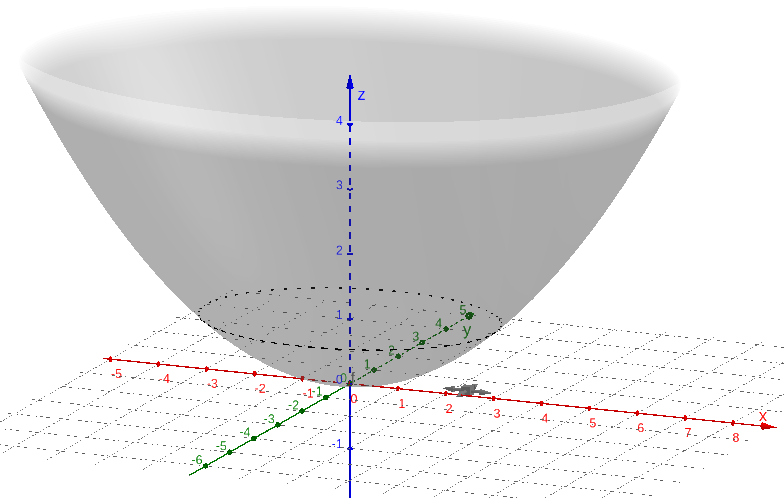
\includegraphics[width=\textwidth]{./cap_superquad/dados/fig_sq_ex_parelip_z/fig}
    \caption{Esboço do paraboloide elíptico de equação \eqref{eq:sq_ex_parelip_z}.}
    \label{fig:sq_ex_parelip_z}
  \end{figure}
\end{ex}

\begin{ex}
  O esboço do gráfico de paraboloide elíptico de equação
  \begin{equation}\label{eq:sq_ex_parelip-x}
    -x = \frac{y^2}{4}+z^2
  \end{equation}
  é dado na Figura \ref{fig:sq_ex_parelip-x}. Verifique!

    \begin{figure}[H]
    \centering
    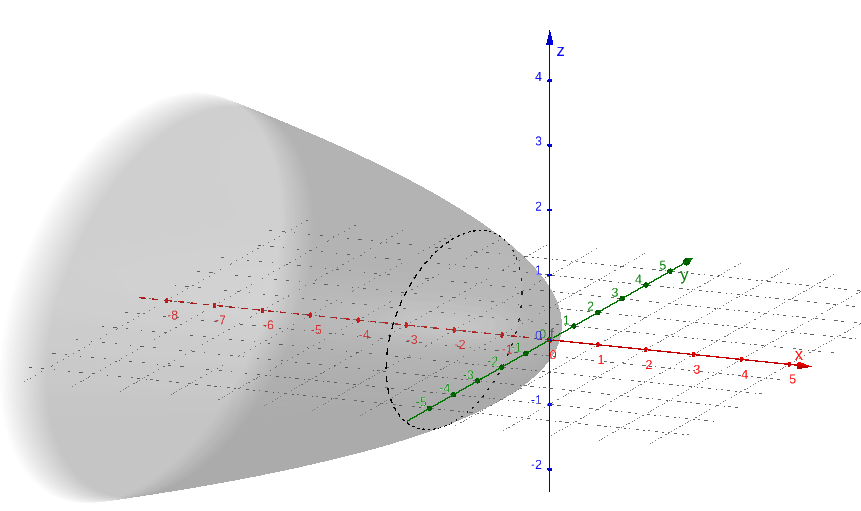
\includegraphics[width=\textwidth]{./cap_superquad/dados/fig_sq_ex_parelip-x/fig}
    \caption{Esboço do paraboloide elíptico de equação \eqref{eq:sq_ex_parelip-x}.}
    \label{fig:sq_ex_parelip-x}
  \end{figure}
\end{ex}

\subsection{Paraboloide hiperbólico}

Um paraboloide elíptico tem equação
\begin{equation}
  \pm z = \frac{x^2}{a^2} - \frac{y^2}{b^2}
\end{equation}
ou
\begin{equation}
  \pm y = \frac{x^2}{a^2} - \frac{z^2}{c^2}
\end{equation}
ou
\begin{equation}
  \pm x = \frac{y^2}{b^2} - \frac{z^2}{c^2}
\end{equation}

\begin{ex}
  Vamos considerar o paraboloide hiperbólico de equação
  \begin{equation}\label{eq:sq_ex_parhiper_z}
    z=\frac{x^2}{9}-\frac{y^2}{4}.
  \end{equation}
  Sua interseção com o plano $X-Y$ ($z=0$) são retas que satisfazem a equação
  \begin{equation}
    \frac{x^2}{9}-\frac{y^2}{4}=0.
  \end{equation}
  De fato, isolando $y$, obtemos as equações destas retas
  \begin{equation}
    y = \pm \frac{2}{3}x.
  \end{equation}
  Sua interseção com o plano $X-Z$ (y=0) é a parábola de equação
  \begin{equation}
    z=\frac{x^2}{9}.
  \end{equation}
  E, a interseção do paraboloide hiperbólico com o plano $Y-Z$ ($x=0$) é a parábola de equação
  \begin{equation}
    z=-\frac{y^2}{4}.
  \end{equation}
  
  A Figura \ref{fig:sq_ex_parhiper_z} é o esboço do gráfico do paraboloide hiperbólico de equação \eqref{eq:sq_ex_parhiper_z}.

    \begin{figure}[H]
    \centering
    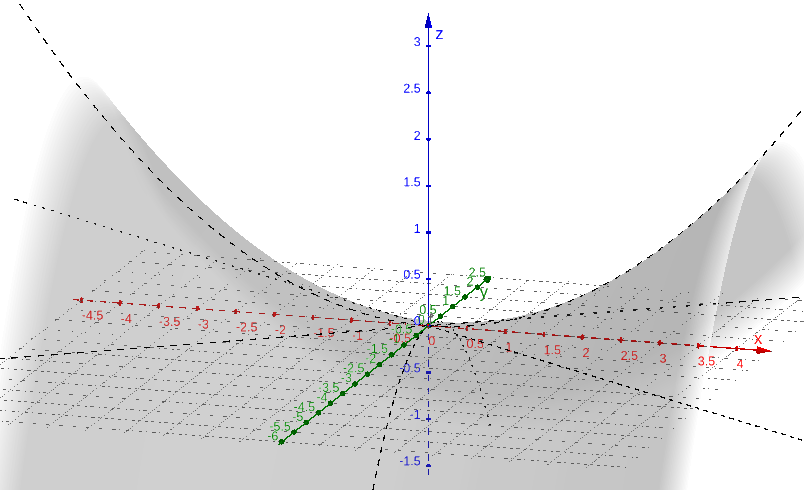
\includegraphics[width=\textwidth]{./cap_superquad/dados/fig_sq_ex_parhiper_z/fig}
    \caption{Esboço do paraboloide hiperbólico de equação \eqref{eq:sq_ex_parhiper_z}.}
    \label{fig:sq_ex_parhiper_z}
  \end{figure}
\end{ex}

\subsection*{Exercícios resolvidos}

\begin{exeresol}
  Escreva a equação do elipsoide que tem como interseções
  \begin{enumerate}[a)]
  \item com o plano $z=0$ a elipse
    \begin{equation}
      \frac{x^2}{4}+\frac{y^2}{16} = 1
    \end{equation}
  \item com o plano $y=0$ a elipse
    \begin{equation}
      \frac{x^2}{4}+\frac{z^2}{9} = 1
    \end{equation}
  \end{enumerate}
\end{exeresol}
\begin{resol}
  Um elipsoide tem equação
  \begin{equation}
    \frac{x^2}{a^2}+\frac{y^2}{b^2}+\frac{z^2}{c^2}=1.
  \end{equation}
  Sua interseção com o plano $X-Y$ ($z=0$) é a elipse de equação
  \begin{equation}
    \frac{x^2}{a^2}+\frac{y^2}{b^2}=1.
  \end{equation}
  Logo, do item a), temos $a^2=4$ e $b^2=16$.

  Agora, a interseção com o plano $X-Z$ ($y=0$) é a elipse de equação
  \begin{equation}
    \frac{x^2}{a^2}+\frac{z^2}{c^2}=1.
  \end{equation}
  Assim, do item b), obtemos $c^2=9$.

  Desta forma, concluímos que o elipsoide de equação
  \begin{equation}
    \frac{x^2}{4}+\frac{y^2}{16}+\frac{z^2}{9}=1.
  \end{equation}
\end{resol}

\begin{exeresol}
  Encontre a equação do paraboloide elíptico que contem a circunferência
  \begin{equation}
    x^2+z^2=1,\quad y=-2.
  \end{equation}
\end{exeresol}
\begin{resol}
  Para que o paraboloide contenha a circunferência
  \begin{equation}
    x^2+z^2=1,\quad y=-2,
  \end{equation}
  ele precisa abrir-se no sentido negativo na direção $y$. Logo, tem equação
  \begin{equation}
    -y = \frac{x^2}{a^2}+\frac{z^2}{b^2}.
  \end{equation}
  Fixado $y=-2$, a equação fica restrita a
  \begin{equation}
    2  = \frac{x^2}{a^2}+\frac{z^2}{b^2}.
  \end{equation}
  Notamos que para esta equação coincida com a circunferência $x^2+z^2=1$, devemos escolher $a^2=b^2=1/2$. Logo, concluímos que o paraboloide elíptico tem equação
  \begin{equation}
    -y = \frac{x^2}{\frac{1}{2}}+\frac{z^2}{\frac{1}{2}}.
  \end{equation}
\end{resol}

\subsection*{Exercícios}

\begin{exer}
  Classifique cada uma das seguintes superfícies quádricas:
  \begin{enumerate}[a)]
  \item $\displaystyle \frac{x^2}{2}-y^2+\frac{z^2}{4}=1$
  \item $\displaystyle x^2+\frac{y^2}{9}+\frac{z^2}{4}=1$
  \item $\displaystyle z = -x^2-\frac{y^2}{9}$
  \item $\displaystyle x^2 + y^2 + z^2 = 0$
  \end{enumerate}
\end{exer}
\begin{resp}
  a) hiperboloide de uma folha; b) elipsoide; c) paraboloide elíptico; d) ponto $(0, 0, 0)$
\end{resp}

\begin{exer}
  Forneça a equação do elipsoide que contem os pontos $P=(0,2,0)$, $Q=(-1,0,0)$ e $R=(0,0,1)$.
\end{exer}
\begin{resp}
  $\displaystyle x^2+\frac{y^2}{4}+z^2=1$
\end{resp}

\begin{exer}
  Forneça a equação do hiperboloide de duas folhas que tem interseções:
  \begin{enumerate}[a)]
  \item com o eixo $X-Y$ igual a hipérbole
    \begin{equation}
      -\frac{x^2}{16}+\frac{y^2}{4}=1
    \end{equation}
  \item com o eixo $Y-Z$ igual a hipérbole
    \begin{equation}
      \frac{y^2}{4}-\frac{z^2}{9}=1
    \end{equation}
  \end{enumerate}
\end{exer}
\begin{resp}
  $\displaystyle -\frac{x^2}{16}+\frac{y^2}{4}-\frac{z^2}{9}=1$
\end{resp}

\begin{exer}
  Forneça a equação do paraboloide elíptico que contem a elipse
  \begin{equation}
    \frac{x^2}{2}+z^2=1,\quad y=2.
  \end{equation}
\end{exer}
\begin{resp}
  $\displaystyle y = x^2+\frac{z^2}{\frac{1}{2}}$
\end{resp}

\begin{exer}
  Considere o hiperboloide de uma folha de equação
  \begin{equation}
    \frac{x^2}{9}-\frac{y^2}{4}+z^2=1.
  \end{equation}
  Classifique o lugar geométrico de sua interseção com cada um dos seguintes planos
  \begin{enumerate}
  \item $X-Y$
  \item $X-Z$
  \item $Y-Z$
  \end{enumerate}
\end{exer}
\begin{resp}
  a) hipérbole; b) elipse; c) hipérbole
\end{resp}
